\chapter{Relevant software technologies} \label{chap:relevant-sofware-technologies}



\section*{}

Robot self-localization in complex environments is a multidisciplinary problem that requires advanced computer software systems. In order to speed up the implementation and deployment of the localization system, several frameworks and libraries were used. Among the most important were \gls{ros} for the system architecture, \gls{pcl} for the point cloud processing and Gazebo for simulation and testing.



\section{\glsentrytext{ros}}

\begin{wrapfigure}{r}{0.25\textwidth}
	\centering
	\includegraphics*[width=0.24\textwidth]{relevant_sofware_technologies/ros_logo}
	\caption{\glsentrytext{ros} logo}
	\label{fig:relevant-sofware-technologies_ros-logo}
\end{wrapfigure}

\gls{ros}\footnote{\url{http://www.ros.org/}} \cite{Quigley2009} is a software framework designed to ease the development of robot systems. It provides seamless integration between hardware drivers and software modules, allowing a fast transition between simulation and deployment.

It's an open source project that offers a distributed computing framework with several core libraries and development tools that aims to speedup software prototyping, testing and deployment.


\subsection{Architecture}

The \gls{ros} architecture was designed from the beginning to be a distributed peer-to-peer software framework that could be deployed in several operating systems and implemented in a range of different programming languages. However, given that most of the \gls{ros} community prefers open source software, the Ubuntu\footnote{\url{http://www.ubuntu.com/}}] operating system is the main developing and testing environment, and as such, the recommended choice for \gls{ros} developers. Moreover, considering that robotics research requires software with both performance and maintainability at its core, the C++\footnote{\url{http://www.cplusplus.com/}} programming language is used in most of the available packages, along with Python\footnote{\url{https://www.python.org/}} and Java\footnote{\url{https://www.java.com}}.

Being a distributed computing framework, \gls{ros} relies in network connections and exchange of messages to perform the intended tasks. As such, its architecture was developed to follow a publish / subscribe pattern (\gls{ros} topics\footnote{\url{http://wiki.ros.org/Topics}}) and request and reply communication paradigm (\gls{ros} services\footnote{\url{http://wiki.ros.org/Services}} and actions\footnote{\url{http://wiki.ros.org/actionlib}}). This allows \gls{ros} nodes\footnote{\url{http://wiki.ros.org/Nodes}} (operating system processes) to be deployed in different computing platforms with ease and simplifies testing and exchange of software modules.

The next sections provide a more detailed description of the main \gls{ros} architecture concepts.


\subsubsection{Nodes}

\gls{ros} nodes are operating system processes that are part of the peer-to-peer communication graph. They are the fundamental building blocks of any \gls{ros} system and can be spread among several computing platforms.

In order to manage the communications between nodes, the \gls{ros} framework provides a master node (roscore\footnote{\url{http://wiki.ros.org/roscore}}) that uses \gls{xmlrpc} to maintain a communication graph of the system. This allows nodes to be started without knowing the location (\gls{ip} address and port) of the other nodes in the network and greatly simplifies their integration and exchange. Also, by using \gls{ros} launch files\footnote{\url{http://wiki.ros.org/roslaunch}} (\gls{xml} configuration files), the specification of a system communication data flow and configuration can be easily altered.

Besides handling communications, the master node also manages system configurations through the parameter server. This allows nodes to share and change the system configuration at runtime. However, given that the parameter server is usually queried only when a node starts up, the dynamic reconfigure\footnote{\url{http://wiki.ros.org/dynamic_reconfigure}} \gls{api} can be used instead, if it is necessary to change the configuration of a node when it is already running. This is achieved by providing a callback that is asynchronously called when a configuration change is requested.

The flexibility provided by \gls{ros} in both module integration and exchange can greatly speedup testing and deployment and the possibility of changing the configuration of the system at runtime and restart software modules individually (nodes) is very useful when implementing system supervisors and recovery behaviors.


\subsubsection{Nodelets}

A nodelet\footnote{\url{http://wiki.ros.org/nodelet}} is a special kind of node that aims to reduce the overhead of message exchange. This overhead can be significant when messages are very large, such as point clouds or video. To mitigate this problem, the nodelets exchange pointers to shared memory regions, instead of sending the entire messages between nodes.

To achieve this overhead reduction, some architecture changes are required. The most important being the use of threads instead of processes, and the creation of a superclass that all nodelets must inherit. This leads to the creation of plugin libraries for each nodelet instead of an executable for each node.

Another important change is the introduction of nodelet managers to allow loading and setup of nodelets in different threads inside the same process.

In terms of implementation, the transition from nodes to nodelets requires few code changes and can lead to a significant improvement of the overall system performance.


\subsubsection{Topics}

\gls{ros} topics are named communication buses that follow the publish / subscribe pattern. They provide a simple method for exchanging messages between nodes and allow the decoupling of information production and consumption. This is useful when there are multiple sources of the same information or there are multiple consumers that are interested in processing the same data for different purposes. Moreover, this communication architecture allows to log and replay the exchanged messages, which can be helpful to test different algorithms with the same data.

Currently, topics can use either the \gls{tcp} or \gls{udp} protocols to exchange messages. The \gls{tcp} implementation is used by default and creates a bidirectional channel between each producer and subscriber while guaranteeing the delivery of all messages. The \gls{udp} implementation uses an unreliable and stateless transport approach, in which a subscriber listens to a given broadcast address, and has no guarantee that will receive all messages. As such, \gls{tcp} should be used when all messages must be processed, and \gls{udp} should be considered when the latency and the \gls{tcp} overhead are important issues.


\subsubsection{Services}

\gls{ros} services are named communication buses that follow the request and reply paradigm, in which a node asks for a given service and receives a response according to the data that was sent in the request message and the state of the service node. They are useful to query other nodes state or to request the execution of some behavior / action.


\subsubsection{Actions}

\gls{ros} actions are a special kind of service in which the progress of the request can be queried. They are very useful when the request might take a long time, and gives the caller the necessary information to supervise the execution of the request and if necessary, terminate its execution.


\subsection{Build system}

The latest \gls{ros} build system is named catkin\footnote{\url{http://wiki.ros.org/catkin}}, and is the successor of the original rosbuild\footnote{\url{http://wiki.ros.org/rosbuild}} system. It combines CMake\footnote{\url{http://www.cmake.org/}} macros and Python scripts to allow building multiple dependent projects at the same time. It is a cross-platform build system, organized in packages and meta-packages (group of packages). Each package is a software module that can produce libraries or binaries from source code.

Catkin was designed to deal with complex build configurations, which in the case of \gls{ros} packages involves a considerable amount of build dependencies for each project. As such, catkin provides a build system that can easily find, build and link both \gls{ros} and system dependencies. Moreover, it provides install targets to allow faster code releases and simplifies builds from source for the final users.

Other useful features of the catkin build system are the concepts of workspace and overlays. Catkin uses a workspace with out-of-source builds to keep the source code separate from the build files. This allows the code directory structure to be clean of compiler generated files that are platform dependent. Moreover, it simplifies the concurrent usage of packages (overlay), because catkin gives priority to workspace packages (in relation to system packages). This is particularly useful when it is necessary to modify and test some package that has been released and is installed in the system (without having to uninstall the stable release of that package).

Finally, catkin is a cross-platform build system that can be used to build other projects that use CMake and are not related to \gls{ros}.


\subsection{Development tools}

\gls{ros} provides several development tools that allow introspection and visualization of the system state. They are very useful for testing, debugging and profiling.

The next sections give an overview of the most important \gls{ros} tools that are currently available.


\subsubsection{Graphical User Interface tools}

The \gls{ros} development tools that have graphical user interfaces are aggregated in the rqt framework\footnote{\url{http://wiki.ros.org/rqt}}, and are loaded as plugins at runtime (some can be started as standalone applications).

Currently there is plugins to visualize sensor data (rviz\footnote{\url{http://wiki.ros.org/rviz}}); introspect the contents of topics; log and replay \gls{ros} messages (rosbag\footnote{\url{http://wiki.ros.org/rosbag}}); display node, package and coordinate systems graphs; list and filter debug messages; change configuration of running nodes (dynamic reconfigure); monitor nodes memory and processor usage and much more.


\subsubsection{Command line tools}

The \gls{ros} command line tools\footnote{\url{http://wiki.ros.org/ROS/CommandLineTools}} are split across several executables and can be used for advanced introspection (rosnode, rostopic and rosservice), system configuration (rosparam), package building and management (catkin, rosdep and rosinstall) and also to search \gls{ros} message types documentation (rosmsg and rossrv).

Finally, it is available a diagnostics tool (roswtf), that can detect packages / dependencies issues and configuration problems.



\section{Gazebo}

\begin{wrapfigure}{r}{0.25\textwidth}
	\centering
	\includegraphics*[width=0.24\textwidth]{relevant_sofware_technologies/gazebo_logo}
	\caption{Gazebo logo}
	\label{fig:relevant-sofware-technologies_gazebo-logo}
\end{wrapfigure}


Gazebo\footnote{\url{http://gazebosim.org/}} is a 3D multi-robot simulator capable of generating hardware sensor data for different kinds of robots while providing a realistic environment with physics simulation and 3D visualization. It is very useful to speedup testing of algorithms with different types of robots and environments.

\Cref{fig:relevant-sofware-technologies_gazebo-ros-integration} shows how Gazebo can be used instead of a real robot, without requiring any implementation code modification (because it implements the same \gls{ros} interfaces that the hardware drivers use).

%\afterpage{
\begin{figure}[ht]
	\centering
	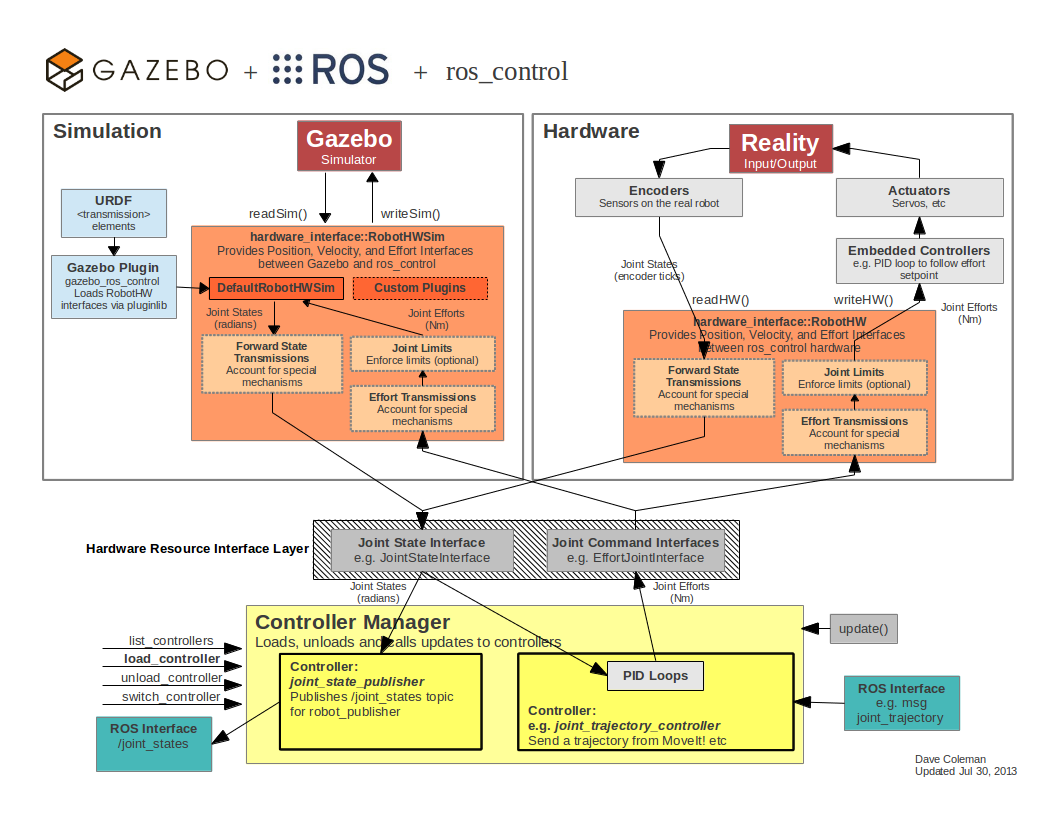
\includegraphics[width=\textwidth]{relevant_sofware_technologies/gazebo_ros_integration}
	\caption[Integration of \glsentrytext{ros} and Gazebo]{Integration of \glsentrytext{ros} and Gazebo\protect\footnotemark}
	\label{fig:relevant-sofware-technologies_gazebo-ros-integration}
\end{figure}
\footnotetext{\url{http://gazebosim.org/tutorials?tut=ros_control}}
%}



\section{\glsentrytext{pcl}}

\begin{wrapfigure}{r}{0.25\textwidth}
	\centering
	\includegraphics*[width=0.24\textwidth]{relevant_sofware_technologies/pcl_logo}
	\caption{\glsentrytext{pcl} logo}
	\label{fig:relevant-sofware-technologies_pcl-logo}
\end{wrapfigure}

The \gls{pcl}\footnote{\url{http://pointclouds.org/}} \cite{Rusu2011} is an open source project that provides algorithms for processing point clouds. These algorithms can be used to filter and register point clouds as well as perform object segmentation, recognition and tracking.

\Cref{fig:relevant-sofware-technologies_pcl-dependency-graph} gives an overview of the main modules currently available in \gls{pcl}.

%\afterpage{
\begin{figure}[ht]
	\centering
	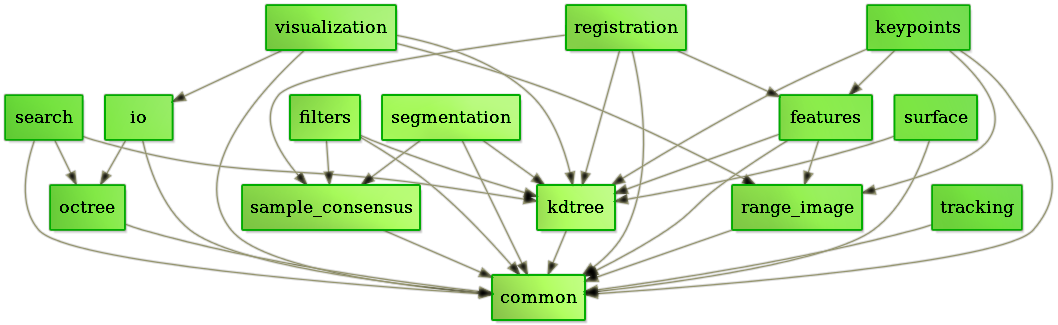
\includegraphics[width=\textwidth]{relevant_sofware_technologies/pcl_dependency_graph}
	\caption[\glsentrydesc{pcl}]{\glsentrydesc{pcl}\protect\footnotemark}
	\label{fig:relevant-sofware-technologies_pcl-dependency-graph}
\end{figure}
\footnotetext{\url{http://pointclouds.org/about/}}
%}
